\documentclass{assignment}
\ProjectInfos{高等热力学与统计物理}{PHYS2110}{2020-2021学年第二学期}{习题 II}{截止时间:2021. 3. 16(周二)}{陈稼霖}{45875852}

\begin{document}
\begin{prob}
    假设热容量 $C_V$ 为常数,求体积为 $V$,温度为 $T$ 的理想气体的熵(确定到一个任意常数)\\
    用所得结果和 Joule 自由膨胀实验论证熵增加原理.
\end{prob}
\begin{sol}
    对于一般系统,熵的全微分可表为
    \begin{align}
        \mathrm{d}S=\frac{C_V}{T}\,\mathrm{d}T+T\left(\frac{\partial P}{\partial T}\right)_V\mathrm{d}V.
    \end{align}
    对上式积分得
    \begin{align}
        \label{1-S}
        S=\int\left[\frac{C_V}{T}\,\mathrm{d}T+\left(\frac{\partial p}{\partial T}\right)_V\mathrm{d}V\right]+S_0,
    \end{align}
    其中 $S_0$ 为一常数.
    对于理想气体,有状态方程
    \begin{align}
        pV=nRT,
    \end{align}
    故
    \begin{align}
        \left(\frac{\partial p}{\partial T}\right)_V=\frac{nR}{V}.
    \end{align}
    将上式代入式 \eqref{1-S},并且假设定容热容量 $C_V$ 为常数,积分得到理想气体的熵为
    \begin{align}
        S=C_V\ln T+nR\ln V+S_0.
    \end{align}
    \emph{用以上结果和 Joule 自由膨胀实验论证熵增加原理}:在 Joule 自由膨胀实验中,气体自由膨胀,同时并不改变温度,也没有吸放热,故在此过程中
    \begin{align}
        \int_{(T_0,V_0)(\text{自由膨胀})}^{(T_0,V)}\frac{\delta Q}{T}=0.
    \end{align}
    假设气体的温度为 $T_0$,膨胀前体积为 $V_0$,膨胀后体积为 $V$,则自由膨胀前气体的熵为
    \begin{align}
        S(T_0,V_0)=C_V\ln T_0+nR\ln V_0+S_0.
    \end{align}
    膨胀后气体的熵为
    \begin{align}
        S(T_0,V)=C_V\ln T_0+nR\ln V+S_0.
    \end{align}
    膨胀前后气体的熵的变化值为
    \begin{align}
        S(T_0,V)-S(T_0,V_0)=nR\ln\frac{V}{V_0}.
    \end{align}
    气体自由膨胀是一绝热的不可逆过程,在此过程中
    \begin{align}
        \int_{(T_0,V_0)(\text{自由膨胀})}^{(T_0,V)}\frac{\delta Q}{T}=0<S(T_0,V)-S(T_0,V_0)=nR\ln\frac{V}{V_0},
    \end{align}
    即末状态的熵高于初状态的熵,
    \begin{align}
        S(T_0,V)>S(T_0,V_0).
    \end{align}
    这论证了熵增加原理 --- 一个绝热系统的熵永远不会降低.
\end{sol}

\begin{prob}
    某一物质具有下列性质:
    \begin{itemize}
        \item[(i)] 在恒定温度 $T_0$ 下体积从 $V_0$ 膨胀到 $V$ 所做的功为
        \[
            W=RT_0\ln\frac{V}{V_0}.
        \]
        \item[(ii)] 该物质的熵由下式给出
        \[
            S=R\frac{V}{V_0}\left(\frac{T}{T_0}\right)^a.
        \]
        其中 $T_0$, $V_0$ 和 $a$ 为固定常数.
    \end{itemize}
    \begin{itemize}
        \item[1)] 计算该物质的 Helmholtz 自由能.
        \item[2)] 求该物质的状态方程.
        \item[3)] 求在任意恒定温度 $T$ 下体积从 $V_0$ 膨胀到 $V$ 所做的功.
    \end{itemize}
\end{prob}
\begin{sol}
    \begin{itemize}
        \item[1)] 自由能的全微分可表为
        \begin{align}
            \mathrm{d}F=-S\,\mathrm{d}T-P\,\mathrm{d}V.
        \end{align}
        由于自由能为一状态量,其变化仅与初末状态有关,而与演化路径无关. 该物质从状态 $(T_0,V_0)$ 等温膨胀至状态 $(T_0,V_0)$,自由能变化
        \begin{align}
            \label{2-DeltaF-1}
            F(T_0,V)-F(T_0,V_0)=\int_{(T_0,V_0)}^{(T_,V)}\mathrm{d}F=-\int_{V_0}^VP\,\mathrm{d}V'=-W=-RT_0\ln\frac{V}{V_0}.
        \end{align}
        从状态 $(T_0,V)$ 定容升温至 $(T,V)$,自由能变化
        \begin{align}
            \label{2-DeltaF-2}
            F(T,V)-F(T_0,V)=\int_{(T_0,V)}^{(T,V)}\mathrm{d}F=-\int_{T_0}^TS\,\mathrm{d}T'=-\int_{T_0}^TR\frac{V}{V_0}\left(\frac{T'}{T_0}\right)^a\,\mathrm{d}T'=-\frac{R}{a+1}\frac{V}{V_0}\left(\frac{T^{a+1}}{T_0^a}-T_0\right).
        \end{align}
        联立式 \eqref{2-DeltaF-1} 与 \eqref{2-DeltaF-2},消去中间态 $(T_0,V)$ 的自由能 $F(T_0,V)$,得
        \begin{align}
            F(T,V)=F(T_0,V_0)-RT_0\ln\frac{V}{V_0}-\frac{R}{a+1}\frac{V}{V_0}\left(\frac{T^{a+1}}{T_0^a}-T_0\right).
        \end{align}
        \item[2)] 自由能对体积求偏导即得状态方程
        \begin{align}
            P=-\left(\frac{\partial F}{\partial V}\right)_T=\frac{RT}{V}+\frac{R}{a+1}\frac{1}{V_0}\left(\frac{T^{a+1}}{T_0^a}-T_0\right).
        \end{align}
        \item[3)] 在任意恒定温度 $T$ 下体积从 $V_0$ 膨胀到 $V$ 所做的功为
        \begin{align}
            \notag W=&-\int_{V_0}^VP\,\mathrm{d}V=-\int_{V_0}^V\left[\frac{RT}{V}+\frac{R}{a+1}\frac{1}{V_0}\left(\frac{T^{a+1}}{T_0^a}-T_0\right)\right]\,\mathrm{d}V\\
            =&-RT\ln\frac{V}{V_0}-\frac{R}{a+1}\left(\frac{V}{V_0}-1\right)\left(\frac{T^{a+1}}{T_0}-T_0\right).
        \end{align}
    \end{itemize}
\end{sol}

\begin{prob}
    一热机循环如右边的 $T-S$ 图所示. 其中 $A$ 代表灰色区域的面积,$B$ 代表灰色区域一下至坐标轴的面积.
    \begin{itemize}
        \item[1)] 证明此热机循环的效率不可能超过可逆循环的效率.
        \item[2)] 证明可逆热机的效率不可能超过工作于最高和最低温度,$T_{\max}$ 和 $T_{\min}$,之间的 Carnot 热机效率.
    \end{itemize}
    \begin{figure}[h]
        \centering
        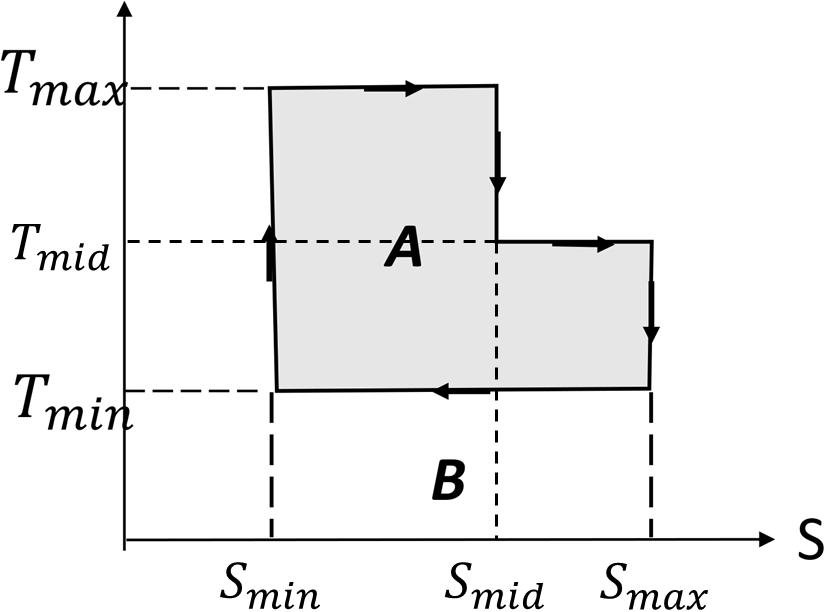
\includegraphics[width=.4\columnwidth]{A2-P3-2.png}
    \end{figure}
\end{prob}
\begin{pf}
    \begin{itemize}
        \item[1)] 对任意一过程(无论可逆与否),总有
        \begin{align}
            \delta Q\leq T\,\mathrm{d}S,
        \end{align}
        其中当且仅当过程为可逆过程时取等号. 假设沿回路的可逆循环吸热 $Q_2$,放热 $Q_1$,沿回路的某个一般循环吸热 $Q_2'$,放热 $Q_1'$,则一般热机的净吸热量低于或等于可逆热机的净吸热量
        \begin{align}
            \oint\delta Q=Q_2'-Q_1'\leq Q_2-Q_1=\oint T\,\mathrm{d}S.
        \end{align}
        对于可逆热机,$\delta Q=T\,\mathrm{d}S$,其仅在灰色区域下边界对应的过程中放热,而一般热机不仅在灰色区域下边界放热(一般热机在这一阶段放出的热量大于可逆热机在这一阶段放出的热量),还可能在其他阶段放热,因此一般热机放出的热量多于或等于可逆热机放出的热量
        \begin{align}
            Q_1'\geq Q_1.
        \end{align}
        从而一般热机 $\eta'$ 的效率不可能超过可逆循环的效率 $\eta$,
        \begin{align}
            \eta'=\frac{Q_2'-Q_1'}{Q_2'}\leq\frac{Q_2-Q_1}{Q_2}=\eta.
        \end{align}
        \item[2)] 如图中所示,设循环中熵的最小值为 $S_{\min}$,最大值为 $S_{\max}$,中间值为 $S_{\text{mid}}$,温度的中间值为 $T_{\text{mid}}$. 可逆热机吸热
        \begin{align}
            Q_1=T_{\min}(S_{\max}-S_{\min}),
        \end{align}
        放热
        \begin{align}
            Q_2=T_{\max}(S_{\text{mid}}-S_{\min})+T_{\text{mid}}(S_{\max}-S_{\text{mid}}).
        \end{align}
        故可逆热机效率为
        \begin{align}
            \eta=\frac{Q_2-Q_1}{Q_2}=1-\frac{T_{\min}(S_{\max}-S_{\min})}{T_{\max}(S_{\text{mid}}-S_{\text{min}})+T_{\min}(S_{\max}-S_{\text{mid}})}.
        \end{align}
        工作于最高和最低温度 $T_{\max}$ 和 $T_{\min}$ 之间的 Carnot 热机效率为
        \begin{align}
            \eta_{\text{Carnot}}=1-\frac{T_{\min}}{T_{\max}}.
        \end{align}
        可逆热机的效率低于 Carnot 热机的效率
        \begin{align}
            \notag\eta=&1-\frac{T_{\min}(S_{\max}-S_{\min})}{T_{\max}(S_{\text{mid}}-S_{\text{min}})+T_{\text{mid}}(S_{\max}-S_{\text{mid}})}\\
            \leq&1-\frac{T_{\min}(S_{\max}-S_{\min})}{T_{\max}(S_{\text{mid}}-S_{\text{min}})+T_{\max}(S_{\max}-S_{\text{mid}})}=1-\frac{T_{\min}}{T_{\max}}=\eta_{\text{Carnot}}.
        \end{align}
    \end{itemize}
\end{pf}

\begin{prob}
    从最小 Gibbs 势的原理而不用 Helmholtz 自由能推导气-液相变的 Maxwell 法则.
\end{prob}
\begin{pf}
    
\end{pf}
\end{document}